\chapter{提案手法}
\label{proposed}



\begin{figure}[hbtp]
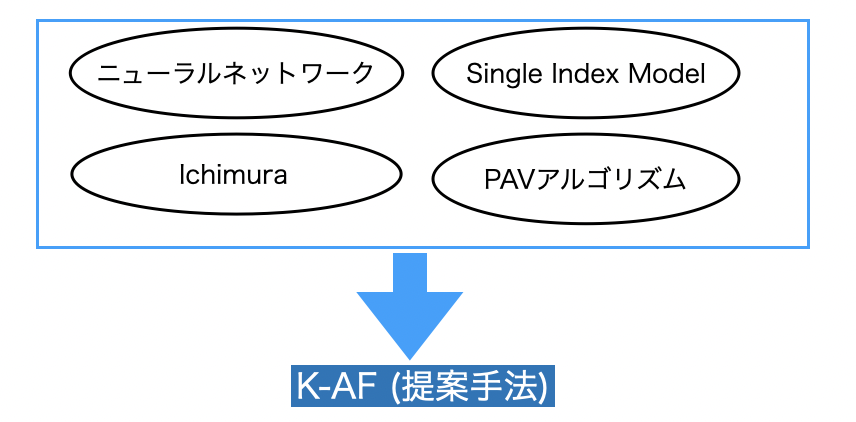
\includegraphics[width=15cm]{asset/proposed_method.png}
	\caption{提案手法}
	\label{proposed_method}
\end{figure}

本章では、まず\ref{mondai}節で本研究が取り組むべき問題を背景を整理しながら述べる。
\ref{mondai}節ではその問題を踏まえ、課題を明確に記す。
\ref{honkadai}節では\ref{kadai}節で述べた課題を解決する本論文の提案手法の歴史と位置付けについて述べる。
\ref{history_activation}節では既存の活性化関数の動向を踏まえながら本提案手法へとつながる過程を述べる。
\ref{position_proposed}節では本研究の研究的な位置付けについて解説する。
\ref{math}節ではK-AFの式について解説し、活性化関数として使用できることを示す。
最後に\ref{al}節ではK-AFのアルゴリズムについて概説し、実装の理解を深める。




\section{問題の背景}
\label {mondai}


現在ニューラルネットワークの構築に使われている活性化関数は組み合わせは問題に応じて、表\ref{which_to_use}のような組み合わせで構築することが多い。

\begin{table}[htbp]
\label{exp:iris}
    \begin{center}
        \caption{問題に応じた活性化関数の選択}
        \label{which_to_use}
        \vspace{2mm} 
        \begin{tabular}{ |c|c|c| }
        問題の種類 & 入力層に使う活性化関数 & 出力層に使う活性化関数\\
        \hline
        分類  & ReLUなど & Sigmoidなど \\
        \hline
        回帰  & ReLUなど & ReLUなど \\
        \hline
        \end{tabular}
    \end{center}
\end{table}

しかし、これらの組み合わせは経験的であるという問題を抱えているだけではなく、問題やデータに対する人間の知識が事前に必要とされる。


\section{本研究が取り組むべき課題}
\label{honkadai}

第\ref{background}章より、活性化関数は今もなお汎用的で精度が向上するような手法が模索されている。
また、これまで用いてきた活性化関数が問題に対して最適だったか確認する手立てが求められている。
本研究ではそれを踏まえて以下の2つの課題に取り組む。

\begin{itemize}
  \item 高い汎用度で活性化関数が自動で推論でき、既存のものより安定的で精度がよくなること。
  \item 関数全体から活性化関数が推定でき、扱っていた活性化関数との差分を確認できるようにすること。
\end{itemize}


\section{提案手法の着想点}
\label{history_activation}

\begin{figure}[hbtp]
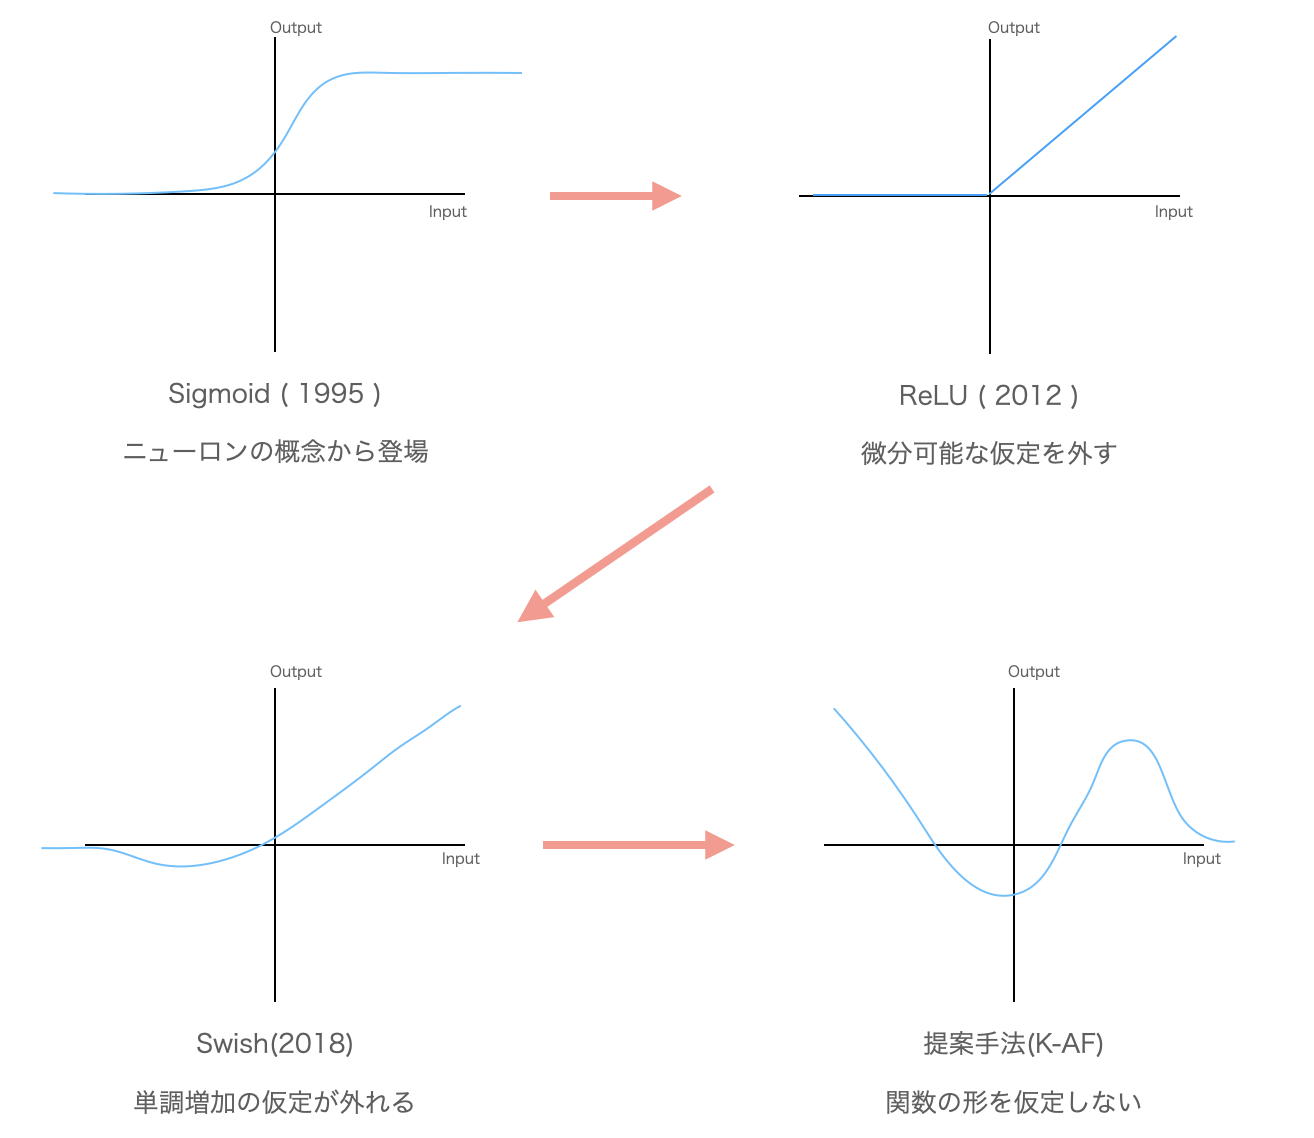
\includegraphics[width=15cm]{asset/history_af.png}
	\caption{活性化関数の歴史}
	\label{history_af}
\end{figure}


本研究で提案する活性化関数はSwishやMishなどからの単調増加性の仮定を外した点に着目した。
Sigmoidはロジスティック回帰から生まれたものであり、ReLU自体も実験的に精度が良いと導出されただけのものであった。
それらの単調増加性という性質は機械学習の観点では本来必要ではないと考えることもできる。
図\ref{history_af}のように、活性化関数はSwishやMishなどといった形へと進化する中で、単調増加性を仮定する必要がなくなった。
isotonic regression同様に単調増加性について仮定しているようであるが、本研究からはその仮定を外す。
そうすることで、より精度の高い結果を導き出すことができると予想される。
関数の推定はカーネル密度推定で行う。
これにより活性化関数を既存の関数から選択するのではなく、関数空間全体から活性化関数を推定することができる。
これにより、これまでディープラーニングで課題とされてきた活性化関数の選択の問題を解決することが可能となり、新たなアプローチが可能になることが予想される。
また、これまで選択してきた活性化関数が実験的に正しいかどうか判定することも可能であると考えられる。


\section{提案手法の位置付け}
\label {position_proposed}

本研究の提案手法の位置付けをまとめた図を\ref{proposed_method}に示した。
統計学の世界でSingleIndexModelにおけるIchimura(1993)の手法を多次元化し、学習アルゴリズムにPAVアルゴリズムを組み合わせた手法をニューラルネットワークの活性化関数に応用する。



\section{K-AF}
\label {math}
本論文で提案する活性化関数を式\ref{eq:k-af}で表現する。

\begin{eqnarray}
G(\mathbf{X}_iw, \mathbf{X}^{calc}, \mathbf{Y}^{calc})=\frac{\sum_{i\neq j} K\left(\frac{\mathbf{X}^{calc}_j w - \mathbf{X}_i w}{h_{calc}}\right)\mathbf{Y}^{calc}_j}{\sum_{i\neq j} K\left(\frac{\mathbf{X}^{calc}_j w - \mathbf{X}_i w}{h_{calc}}\right)}
\label{eq:k-af}
\end{eqnarray}


$ \mathbf{X}^{calc}_j $及び$ \mathbf{Y}^{calc}_j $ は計算用に用いるデータ点である。
現在の機械学習における問題の多くは学習に用いるデータセットが非常に大きい。
そのため、Ichimura(1993)~\cite{ichimura}ではデータセットの数だけで表現していたが、一部を省略することにより少ないデータ点で表現する。
少ないデータ点で記述することは、活性化関数の形の単純化と計算量を減らすことにも直結する。

詳細な式の導出はappendix\ref{appendix:calc}で述べた。


\subsection{バンド幅推定}


\begin{figure}[hbtp]
    \begin{center}
            \begin{minipage}{0.40\hsize}
                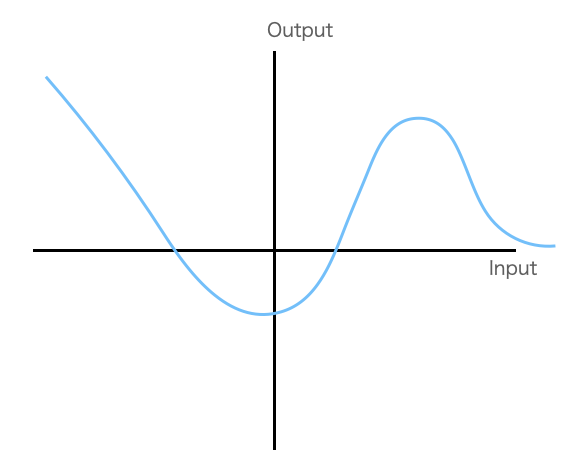
\includegraphics[width=5cm]{asset/k_af_band_big.png}
                    \caption{バンド幅が大きいと、K-AFで表現できる活性化関数の数は減る。}
                    \label{k_af_band_big}
            \end{minipage}
            \begin{minipage}{0.40\hsize}
            \hspace{10pt}
                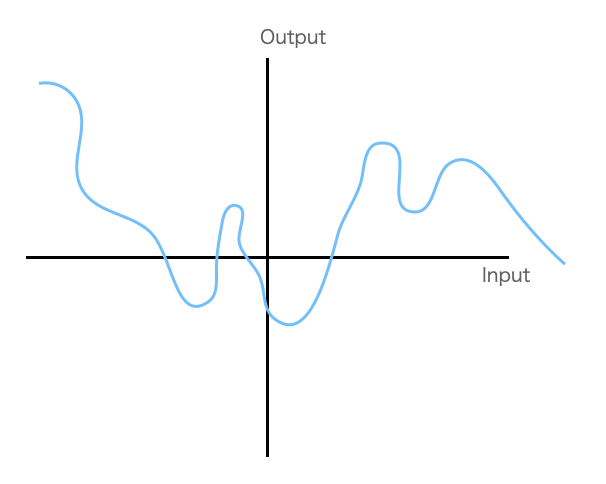
\includegraphics[width=5cm]{asset/k_af_band_small.png}
                    \caption{バンド幅が小さいと、K-AFで表現できる活性化関数の形は大きくなる。}
                    \label{k_af_band_small}
            \end{minipage}
    \end{center}
\end{figure}


カーネル密度推定は関数の形状を推定するにあたってバンド幅の大きさが非常に重要になる。
バンド幅は大きいほど関数の自由度が減り、小さいほど自由度が大きくなることが容易に推定できる。

図\ref{k_af_band_small}の方が表現の幅が広いが、勾配爆発の問題や過学習の問題が考えらる。
本実験ではこのバンド幅も学習のパラメータに含めることで最適なバンド幅を推定できるようにした。

\section{アルゴリズム}
\label{al}
K-AFのアルゴリズムの概要を{\bf Algorithm}\ref{alg:fixed-u-alg}に記述した。

入力の次元を$ d $ 出力の次元を$ e $とする。$ m $をミニバッチのサイズ、$ w^t $を$t$ステップ目の重みのパラメータとする。
また、$x$のデータセットの集合を$ \mathcal{D}_x $ $y$のデータセットの集合を$ \mathcal{D}_y $、それらから$n$個サンプリングすることを$ \mathbf{Y}^{calc} \sim_n \mathcal{D}_y $と記述する。
$ \mathrm{E} $を目的関数とした時、以下のアルゴリズムで最適化を表現することができる。



\begin{algorithm}[]
	\caption{\KAF}
	\label{alg:fixed-u-alg}
\begin{algorithmic}
	\STATE {\bfseries Input:} data $\langle (\mathbf{X}_i, y_i) \rangle_{i=1}^m \in
	\reals^d \times \reals^e$, $G: ( \reals^d, \reals^n, \reals^n ) \rightarrow  \reals^e$.
	\STATE $\mathbf{X}^{calc} \sim_n \mathcal{D}(\mathbf{X})$;
    \STATE $\mathbf{Y}^{calc} \sim_n \mathcal{D}(\mathbf{Y})$;
	\FOR {$t = 1, 2, \ldots$}
	\STATE $g^t(x) := G(\mathbf{X} \cdot  \mathbf{W}^t, \mathbf{X}^{calc}, \mathbf{Y}^{calc} )$;
	\STATE $ \displaystyle{\min_{w} \mathrm{E}(w)} = \frac{1}{2}\sum_m (y_i - g^t(\mathbf{X}_i))^2 $
	\ENDFOR
\end{algorithmic}
\end{algorithm}

\begin{itemize}
  \item データセット$\mathcal{D}_x$,$\mathcal{D}_y$から任意個数の$ \mathbf{X}^{calc} $と$ \mathbf{Y}^{calc} $から取り出す。
  \item 現状のパラメータ$ w $, $\mathcal{D}_x$, $\mathcal{D}_y$を用いて、リンク関数$ g^t $の計算を行う。
  \item そのリンク関数を用いて$ y $の値との最小二乗誤差を取り$ w $に対して最適化を行う。
\end{itemize}


pythonでの実装についてはappendix\ref{appendix:algorithm}に記述した。






%%% Local Variables:
%%% mode: japanese-latex
%%% TeX-master: "../bthesis"
%%% End:
